%
% File: chap02.tex
%
\let\textcircled=\pgftextcircled
\chapter{Graph Partitioning for Large Graphs}
\label{Chapter3}
This chapter is going to develop all the concepts related to the modifications made to the GAP framework. It contains the proposed solution and a description of why some decisions were made.

\section{Node Embeddings}
As mentioned by Zhang et. al.~\cite{gcnreview}, GCN's and its variants have become a very hot topic in Machine Learning and they are being extremely used to solve plenty of problems. Indeed, the use use of Graph Convolutional Networks (GCN) to generate \textit{node embeddings} was a key factor that made the GAP framework very successful in producing good quality partitions. Recall that node embeddings are dense vector representations for the nodes in the involved graph.

Graph Convolutional Networks can solve the following limitations found in traditional encoders~\cite{encoderlimitations}:
\begin{itemize}
    \item Traditional encoders do not scale, they generate unique embeddings for each node.
    \item Traditional approaches can only generate embeddings for a single fixed graph.
    \item They only use the graph structure and they do not consider node features 
    \item Those encoders focus on a specific architecture and cannot be adapted to train with different loss functions.
\end{itemize}

\subsection{Graph Convolutional Networks}
Graph Convolutional Networks were originally proposed by Kifp et. al.~\cite{gcn}. When they first came up with its algorithm, they proposed a model where a single layer follows the following propagation rule:
\begin{align}
    \label{eq:gcn}
    H^{(l+1)} = f(H^{(l)}, A) &= \sigma\left(\hat{D}^{-\frac{1}{2}}\hat{A}\hat{D}^{-\frac{1}{2}}H^{(l)}W^{(l)}\right) \\
    & H^{(0)} = X,
\end{align}
where $\boldsymbol W^{(l)}$ is a the learnable parameter weight matrix for the $l$-th network layer, $\hat{A}=A+I$ is the adjacency matrix with self loops, $\hat{D}$ is the diagonal node degree matrix of $\hat{A}$, $X$ is the feature matrix, and $\sigma$ is a non-linear activation function. Also note that the term $\hat{D}^{-\frac{1}{2}}\hat{A}\hat{D}^{-\frac{1}{2}}$ is a symmetric normalized version of the graph Laplacian.

Although GCN's are extremely powerful to generate node embeddings, in practice they have the following downsides:
\begin{itemize}
    \item GCN's are slow to train. As it can be seen in Equation~\ref{eq:gcn}, they multiply feature matrices by powers of the normalized graph's Laplacian, i.e., they are computationally very expensive. 
    \item GCN's consume a lot of memory when training. They are not suitable for either dense graphs or large graphs.
    \item They present over-smoothing. After stacking multiple rounds of message passing, GCN's contain similar information in all nodes embedding representations~\cite{hamilton}.
\end{itemize}

To solve this issues in GCN's, several solutions have been proposed that deal with the downsides mentioned without loosing the expressibility of the GCN. Some of the most relevant solutions for this work are FastGCN, GraphSAGE and PinSAGE.

FastGCN~\cite{fastgcn} introduces sampling to the GCN framework and reformulate the loss function to provide a mechanism for inductive learning. I address the efficiency problems found in training GCN's by adding a batching training scheme using Monte Carlo techniques. Finally FastGCN shows better generalization than its preceding framework. 

Similar to FastGCN, GraphSAGE~\cite{graphsage} is an inductive version of GCN's. It introduces sampling techniques that remove the dependency of having all nodes during the training stage improving the performance and running time of GCN's. GraphSAGE naturally generalizes to unseen nodes and can learn about the local graph structure.

From all the mentioned solution, PinSAGE~\cite{pinsage} is perhaps the most complete and successful. This is the architecture used by Pinterest for their recommendation system. PinSAGE operates on an enormous graph with $3$ billion nodes and $18$ billion edges. It uses a combination of random walks and a MapReduce-based inference to compute the node embeddings improving dramatically the scalability of GCN's.

For this research, GraphSAGE was chosen due to its flexibility and its superior performance on many graph-related tasks. As its authors suggested~\cite{graphsage}, new sampling techniques can be easily adapted as well as an application-driven loss function. Alternative approaches that can be also adapted to work in the problem in question are described in~\cite{gnnsurvey} or~\cite{hamilton}.

%Mention all the approaches that use Graph Neural Networks and its importance in solving graph related tasks


%Talk a little bit about traditional node embeddings approaches and its delimitations.
%Embeddings: dense vector representations
%Talk about the message passing framework
%Start with Grpah Convolutional Neural Networks (GCN) and its limitations. Emphasize in how GraphSAGE solve those limitations and how it extends the GCN capabilities

\subsection{GraphSAGE}
As claimed by the authors of the paper~\cite{graphsage} where it was first proposed, GraphSAGE is an inductive framework that generate node embeddings for previously unseen data. It can be seen as an extension of the GCN framework to the inductive setting but it results advantageous in this process as it:
\begin{itemize}
    \item Performs localized convolutions without needing to use the whole normalized Laplacian resulting in a reduction of the computing time. Due to the nature of the GCN's, they make use of the symmetrically normalized graph Laplacian localized convolutions.
    \item Does not require that all nodes are present during training of the embeddings which turns out in a highly scalable framework.
    \item Naturally generalize to unseen nodes and even complete sub-graphs.
    \item Is capable of recognizing local and global structural properties of nodes based only on its neighborhood even though it still depends on node features.
    \item Uses an unsupervised loss function that tries to preserve graph structure without being specific on the task.
\end{itemize}

The basic idea of this framework to compute an embedding for node $v$ can be summarized by the following three steps:
\begin{enumerate}
    \item Sample a set of nodes from the neighborhood of $v$ uniformly at random
    \item Aggregate feature information from neighbors
\end{enumerate}

Having this idea in mind, the simplest form of a layer-wise propagation rule for GraphSAGE is given by
\begin{align}
    \label{eq:graphsage}
    \boldsymbol h_v^{(l)} &= \sigma\left(\boldsymbol W^{(l)}\cdot \textsc{Concat}\left(\boldsymbol h_v^{(l-1)},h_{N_l(v)}^{(l)}\right)\right) \nonumber \\
    \boldsymbol h_{N_l(v)}^{(l)} &= \textsc{Aggregate}_l\left(\left\{h_u^{(l-1)} \mid u\in N_l(v)\right\}\right) \\
    \boldsymbol h_v^{(0)} &= \boldsymbol  X_v \nonumber
\end{align}
where as usual $\boldsymbol W^{(l)}$ is a the learnable parameter weight matrix for the $l$-th network layer and $\sigma$ is a non-linear activation function, $\{\boldsymbol X_v \mid v\in V\}$ are the input features, $\textsc{Aggregate}_l$ are differentiable aggregator functions, and $N_l:v\rightarrow 2^V$ are neighborhood sampling functions.

After computing the node embedding for the $l$-th layer, the algorithm also performs a normalization step by dividing by the vector norm. This step is a common technique to prevent gradient explosion.

To learn the GraphSAGE parameters and get useful predictive node representations, the model can be trained in a fully unsupervised manner by using the following graph-based loss function:
\begin{equation}
    \label{eq:sageloss}
    J_G(\boldsymbol z_u) = -\log\left(\sigma(\boldsymbol z_u^T\boldsymbol z_v)\right) - Q\cdot\mathbb{E}_{v_n\sim P_n(v)}\log\left(\sigma(-\boldsymbol z_u^T \boldsymbol z_{v_n})\right) 
\end{equation}

\begin{figure}[h!]
    \begin{center}
        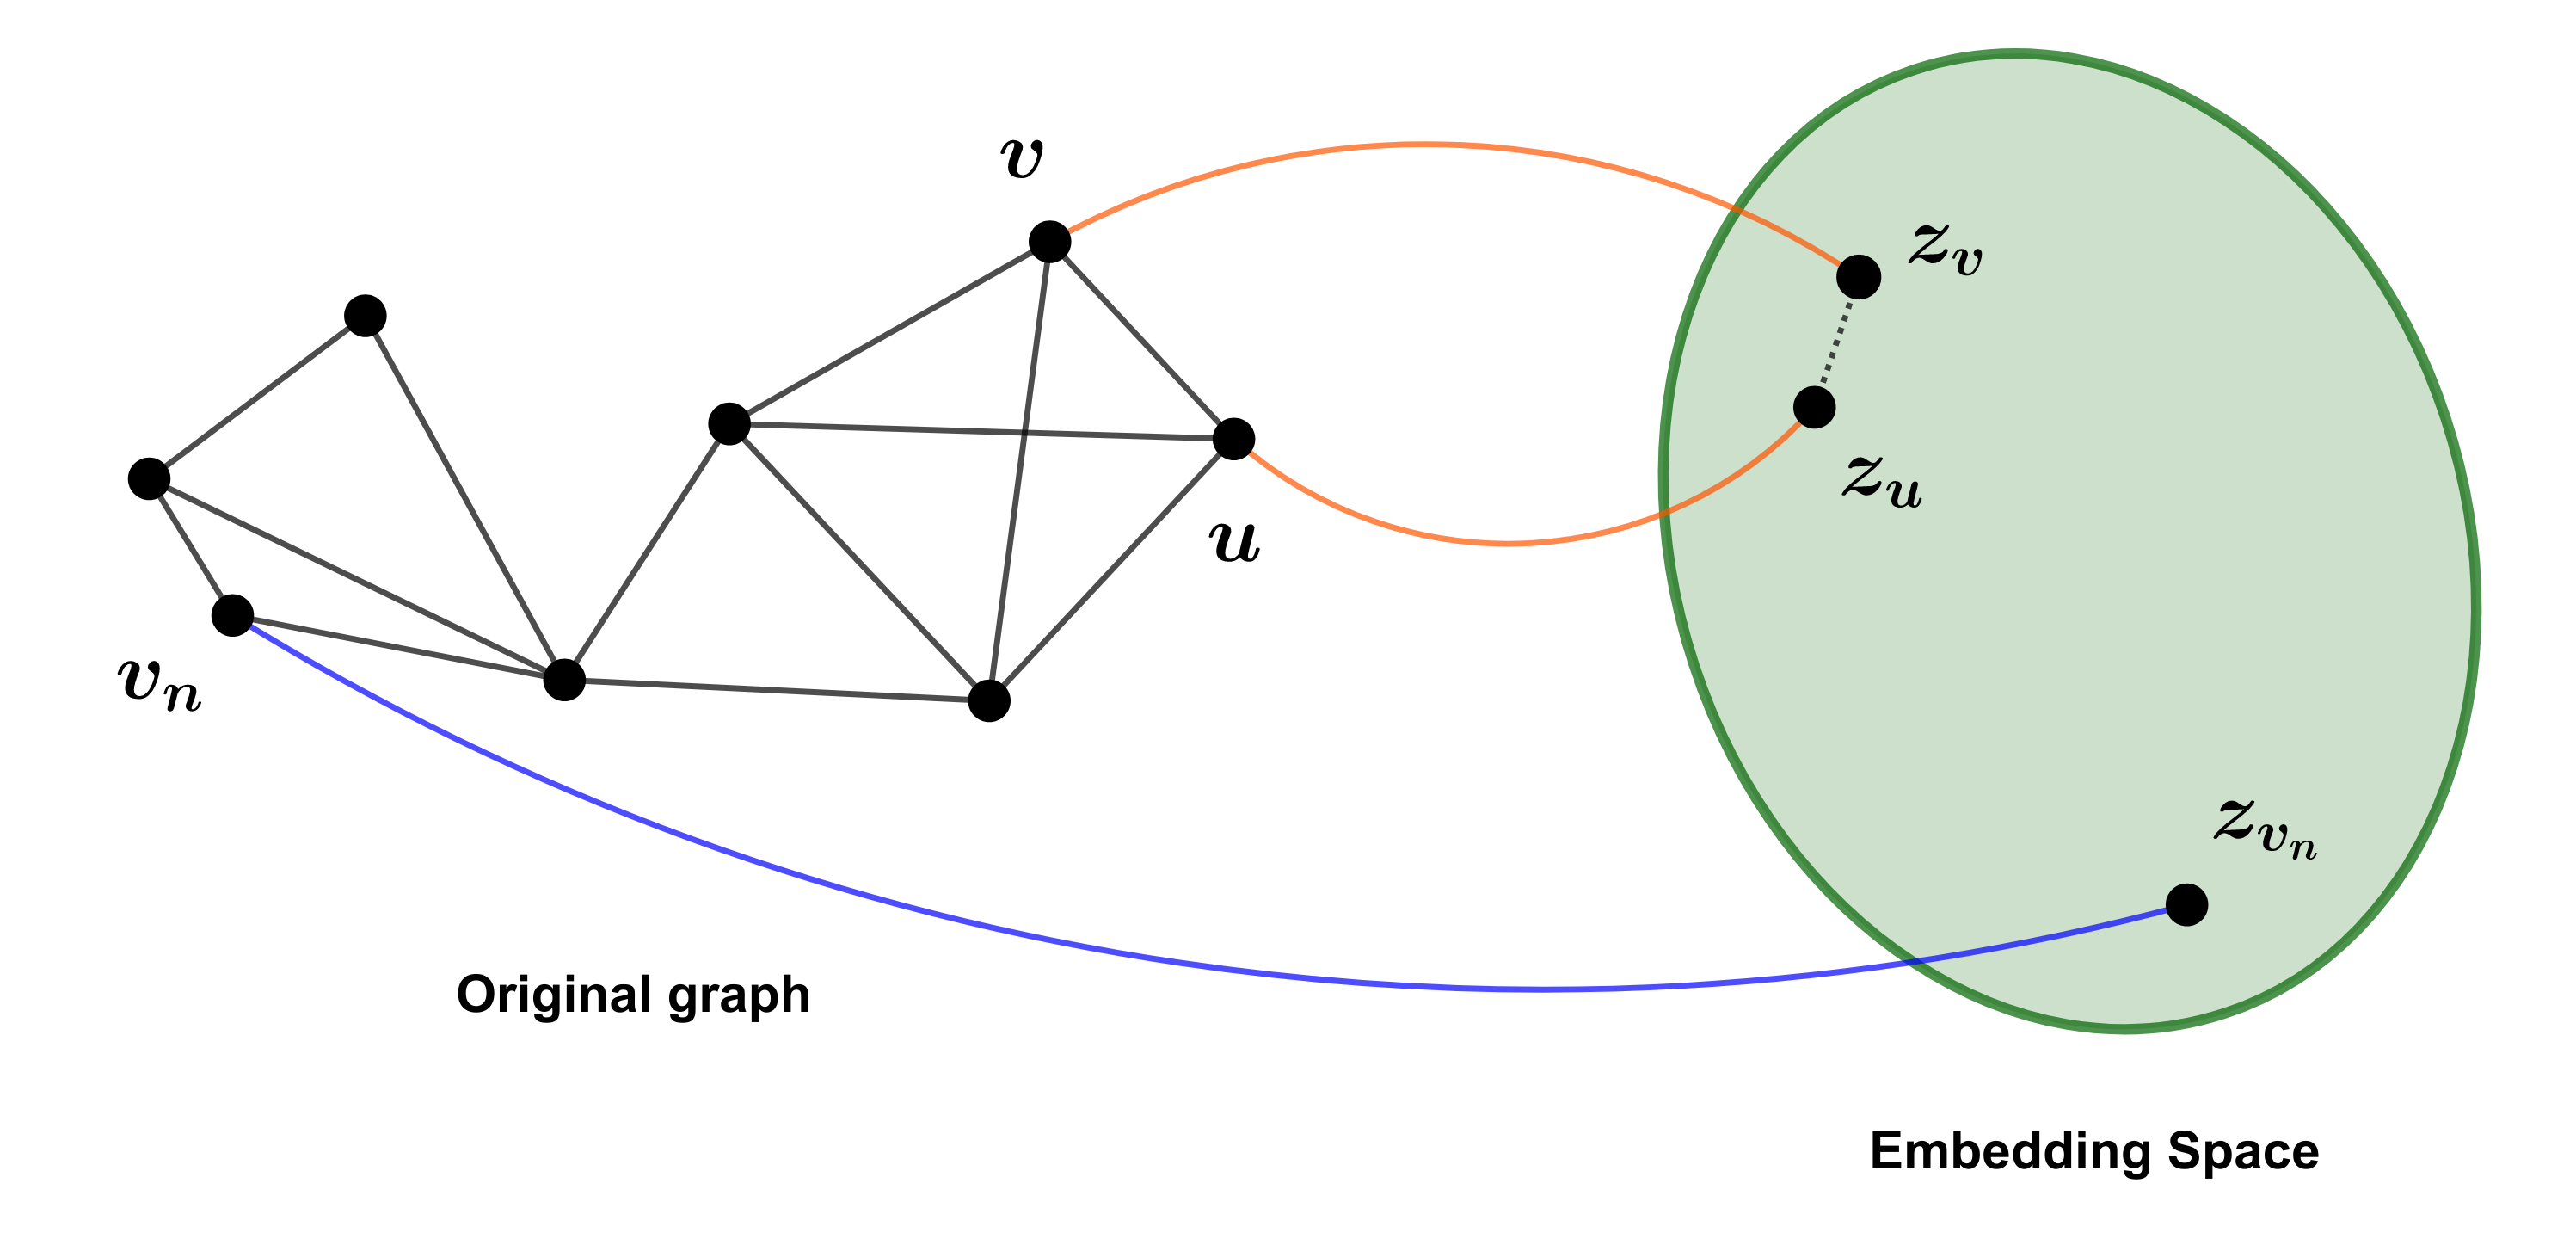
\includegraphics[scale=0.15]{graphSAGE_loss}
    \end{center}
    \caption{Graphical representation of the embeddings generated by GraphSAGE}
    \label{fig:graphsageloss}
\end{figure}

As explained by Abraham~\cite{unsupervisedloss}, the supervised loss function given by Equation~\ref{eq:sageloss} is designed in a way that if nodes $u$ and $v$ are close in the original graph, their node embeddings should be similar. See Figure~\ref{fig:graphsageloss}. 

On one hand, if $u$ and $v$ are close, we expect the inner product of their representations $z_u$ and $z_v$ to be large and the first term of Equation~\ref{eq:sageloss} will be close to zero. On the other hand, if $u$ and $v$ are distant to each other, it is expected that their inner product is negative so the value of the second term will be close to zero. Since all distant nodes, also known as negative nodes, cannot be used to minimize the loss function, only $Q$ of them are sampled from the distribution of negative nodes $P_n(v)$.

%Figure~\ref{fig:graphsageloss} shows a graphical representation on how the GraphSAGE loss function works to generate useful node representations.


\section{Node Features}
For a graph $G = (V,E)$, where $V=\{v_1, v_2, ..., v_n\}$, the feature matrix $X$ can be described as the $n\times F$ matrix where the rows $X_{v_i}$ are node features that depends on the graph. For example, in the context of social networks, node features can be gender, city or any other user profile information.

\begin{figure}[h!]
    \begin{center}
        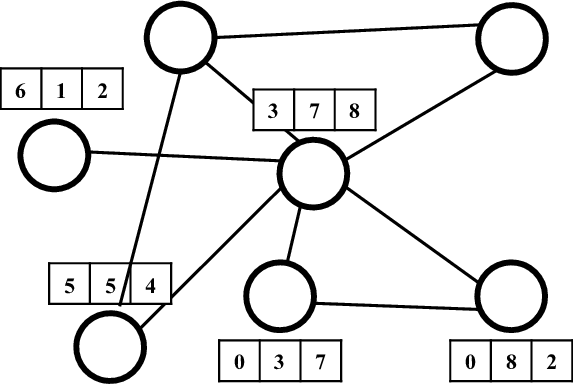
\includegraphics[scale=0.35]{node_features.png}
    \end{center}
    \caption{Graph with $7$ nodes, five of them with $3$ node features~\cite{imagenodefeatures}.}
    \label{fig:nodefeatures}
\end{figure}

Many graphs from different applications come with very rich node feature information that can be very representative in the node embedding generation process. The key idea of Graph Neural Networks is to generate representations of nodes that depends not only on the structure of the graph but from any feature information of the graph. 

As mentioned by Chen Wang et. al.~\cite{nodefeatures}, Graph Neural Networks (GNN's) aim at learning node representations by learning the similarities shared between connected nodes. However, the expressive ability of a GNN is highly dependent on the quality of node features.
 
In the version of the GP problem presented here, node features are irrelevant. The information that nodes or edges could contain does not determine if a node will belong to a specific partition or if an edge will be removed in the partitioned graph. Due to this fact and the inherent characteristic of GCN's before mentioned, one of the main limitations found in the GAP framework is that it requires node features. Furthermore, in specific important GP applications, graphs do not have node features. 

Learning inductive representations on graphs without node features it is still an open problem ~\cite{gnnsurvey}. Nonetheless, for specific applications some efforts have been accomplished which generate new research opportunities. The next paragraphs are dedicated to study the impact of considering different sources of information as node features.

Two of the most common approaches where no node features are available are to use \textit{identity features} and to use random feature initialization. However, those approaches have shown to be equivalent and to make the model incapable of generalizing to unseen nodes~\cite{hamilton}.

\sloppy Another option is to use graph statistics like: node degree, node centrality, number of closed triangles or the clustering coefficient.
Cai and Wang~\cite{nonattributed} proposed a degree-based approach. They used some statistics of the node's degree to generate the node features. Specifically, they used the feature vectors given by $(degree(v), \min(DN(v)), \max(DN(v)), mean((DN(v)), std(DN(v))$ where $DN(v)=\{degree(u)\mid (u,v)\in E\}$. This is an interesting research that showed prominent results.

Other methods propose using applying methods such as PCA to the adjacency matrix to extract the top k-eigenvalues~\cite{eigen, eigen2} but those approaches are computationaly very expensive, which is infeasible for large graphs.

In this work, to help capturing local information related to the graph's structure, a random walk approach was preferred. Given the the existent research, this type of approach looks very promising in terms of scalability to large graphs and structural representation capabilities. In experiments carried out independently by Duong et. al.~\cite{onnodefeatures} and Cui et. al.~\cite{onpositional}, who compared some of the already mentioned approaches, they concluded that matrix-decomposition-based methods are very powerful to extract positional node information. DeepWalk~\cite{deepwalk} produces a low-rank tranformation of the graph's normalized Laplacian matrix~\cite{factorizing}, i.e., DeepWalk is implicitly factorizing and reducing dimensionality. For that reason, DeepWalk is going to be used for this task.

%have been shown efficient representation learning techniques for graphs https://arxiv.org/pdf/1901.01346.pdf, random walk kernels to produce high quality graph representations https://proceedings.neurips.cc/paper/2020/file/ba95d78a7c942571185308775a97a3a0-Paper.pdf

\subsection{DeepWalk as feature extraction}

playing with the parameters

in particular Deep Walk to extract features about the topology of the network

According to the original paper~\cite{deepwalk}, the DeepWalk algorithm consists of two main components: a random walk generator and an update procedure. 

In the first component, a random node $v_i$ is taken uniformly at random to be the root of a random walk $\mathcal W_{v_i}$ which in its turn samples recursively from the neighbors of the last visited vertex until the maximum length $\gamma$ is reached.

Traditional approaches like METIS or SCOTCH implements different versions of the algorithm according to the balancedness measure, either the cardinality or the volume of the partitions. One of the great innovations presented  in~\cite{gap} is the introduction of a loss function derived from the expectation of the normalized cut. Even though they 

Ratio cut it is still used and relevant to modern research cite here https://proceedings.neurips.cc/paper/2020/file/aa108f56a10e75c1f20f27723ecac85f-Paper.pdf

or here https://www.springerprofessional.de/en/metaheuristic-approaches-for-ratio-cut-and-normalized-cut-graph-/20360832    

the authors of~\cite{gap2} proposed some modifications to GAP so it can be used for graphs without features. However the presented 

for future - Study the weighted problem
Study better features related to the problem
other ways to extract useful features for non-attributed graphs

METIS was used from the networkx interface

a table for commonly used notation



\section{Markov Chain Negative Sampling (MCNS)}
